\documentclass[10pt]{beamer}
\usepackage{graphicx}
\usepackage{subfig}
\usepackage{color}
\usepackage{tikz}
	\usetikzlibrary{shapes.geometric, arrows}
	\usetikzlibrary{arrows,shapes,matrix}
	\usetikzlibrary{decorations.pathmorphing} 
	\usepgflibrary{plotmarks}
	\usetikzlibrary{patterns}  
	\usetikzlibrary{positioning} 
	\tikzstyle{roundedRectangle} = [rectangle, rounded corners, minimum width=3cm, minimum height=1cm,text centered, draw=black]
	\tikzstyle{link} = [thick, -]
	\tikzstyle{circleNode} = [circle, minimum size = 1cm, text centered, draw=black, inner sep=0.1cm]
	\tikzstyle{solidNode} = [circle,fill,inner sep=1pt]
	\tikzstyle{startstop} = [rectangle, rounded corners, minimum width=3cm, minimum height=1cm,text centered, draw=black]
	\tikzstyle{io} = [trapezium, trapezium left angle=70, trapezium right angle=110, minimum width=3cm, minimum height=1cm, text centered, draw=black]
	\tikzstyle{process} = [rectangle, minimum width=2cm, minimum height=1cm, text centered, draw=black, inner sep=0.1cm]
	\tikzstyle{decision} = [diamond, minimum width=2cm, minimum height=0cm, text centered, draw=black, inner sep=0cm]
	\tikzstyle{arrow} = [thick,->,>=stealth]
	\tikzstyle{branchnode} = [circle, minimum size = 1cm, text centered, draw=black, inner sep=0.1cm]
\usetheme{Copenhagen}

\title{Gurobi Workshop - Part I}
\author{Lan Peng, PhD Candidate}
\institute{Department of Industrial \& Systems Engineering\\University at Buffalo, SUNY}
\date{\today}

\begin{document}
	\begin{frame}[plain]
		\titlepage
	\end{frame}

	\begin{frame}
		\frametitle{Overview}
		\begin{itemize}
			\item Part I - 26th Oct.
			\begin{itemize}
				\item Introduction and Installation
				\item Manufactures Problem - Small Example of LP
				\item Parallel Machine Scheduling Problem - Simple Example of IP
				\item Traveling Salesman Problem - Lazy Constraints and Callback
			\end{itemize}
			\item Part II - 2nd Nov.
			\begin{itemize}
				\item Vehicle Routing Problem with Time Windows - Column Generation
				\item Facility Location Problem - Benders Decomposition
			\end{itemize}
		\end{itemize}
	\end{frame}

	\section{Introduction and Installation}
		\begin{frame}
			\frametitle{Introduction}
			\begin{itemize}
				\item Gurobi $\rightarrow$ Dr. Gu, Dr. Rothberg, Dr. Bixby.
				\item The best MIP solver (for now).
				\item Can be integrated into Python, C++, Java, Matlab, etc.
				\item Homepage: \textcolor[rgb]{0,0,1}{\url{https://www.gurobi.com/}}
			\end{itemize}			
		\end{frame}

		\begin{frame}
			\frametitle{Installation}
			\begin{itemize}
				\item 1. To download gurobi, we will need to sign up for an account on \textcolor[rgb]{0,0,1}{\url{https://pages.gurobi.com/registration}}. Remember that we need to use the .edu email address to get the free education license.
				\item 2. Then, we can find the distribution on the following link: \textcolor[rgb]{0,0,1}{\url{https://www.gurobi.com/downloads/gurobi-software/}} (login required). This page has many different versions for different OS.
				\item 3. The next step will be getting a license, which we can get from \textcolor[rgb]{0,0,1}{\url{https://www.gurobi.com/downloads/end-user-license-agreement-academic/}} (login required).
				\item 4. After we retrieved the license, we can use the terminal command to execute the \textcolor[rgb]{0.7,0.7,0}{`\texttt{grbgetkey YOUR\_LICENSE}`} to activate the license.
				\item 5. In terminal, go to the root direction of Gurobi, run \textcolor[rgb]{0.7,0.7,0}{`\texttt{python setup.py install}`}.
				\item 6. If all those steps are done, we can now try to import gurobi in python using \textcolor[rgb]{0.7,0.7,0}{`\texttt{import gurobipy}`}.
			\end{itemize}
		\end{frame}

	\section{Manufactures Problem}
		\begin{frame}
			\frametitle{Manufactures Problem}
				\textbf{Manufactures Problem} Giapetto’s Woodcarving, Inc., manufactures two types of wooden toys: soldiers and trains. A soldier sells for \$3 of profit and a train sells for \$2 of profit. The manufacture of wooden soldiers and trains requires two types of skilled labor: carpentry and finishing. A soldier requires 2 horus of finishing labor and 1 hour of carpentry labor. A train requires 1 hour of finishing and 1 hour of carpentry labor. Each week, Giapetto can obtain all the needed raw materials but only 100 finishing hours and 80 carpentry hours. Demand for trains is unlimited, but at most 40 soldiers are bought each week. Giapetto wants to maximie weekly profit. Formulate a mathematical model to Fiapetto’s situation that can be used to maximize Giapetto’s weekly profit.
		\end{frame}

		\begin{frame}
			\frametitle{Manufactures Problem}
			- \textbf{Decision Variable:}
			\begin{itemize}
				\item $x_1$ - Number of soldiers
				\item $x_2$ - Number of trains
			\end{itemize}

			- \textbf{Linear Programming Model:}
			\begin{align}
				\max \quad & 3 x_1 + 2 x_2 \label{p1:obj:maxProfit}\\
				\text{s.t.} \quad & 2 x_1 + x_2 \le 100 \label{p1:con:finishing}\\
				& x_1 + x_2 \le 80 \label{p1:con:carpentry}\\
				& x_1 \le 40 \label{p1:con:atmost}\\
				& x_1, x_2 \ge 0 \label{p1:con:neg}
			\end{align}

			- \textbf{Objective Function: }
				(\ref{p1:obj:maxProfit}) - maximize profit

			- \textbf{Constraints:}
			\begin{itemize}
				\item (\ref{p1:con:finishing}) - Total finishing labor hours
				\item (\ref{p1:con:carpentry}) - Total carpentry labor hours
				\item (\ref{p1:con:atmost}) - at most 40 soldiers are brought
				\item (\ref{p1:con:neg}) - Non-negativity constraints.
			\end{itemize}
		\end{frame}

	\section{Parallel Machine Scheduling Problem}
		\begin{frame}
			\frametitle{Parallel Machine Scheduling Problem}
			Given $n$ jobs $j_1, j_2, \cdots, j_n$ of varying processing times, which need to be scheduled on $m$ machines while trying to minimize the makespan
			\begin{figure}[!h]
				\centering
				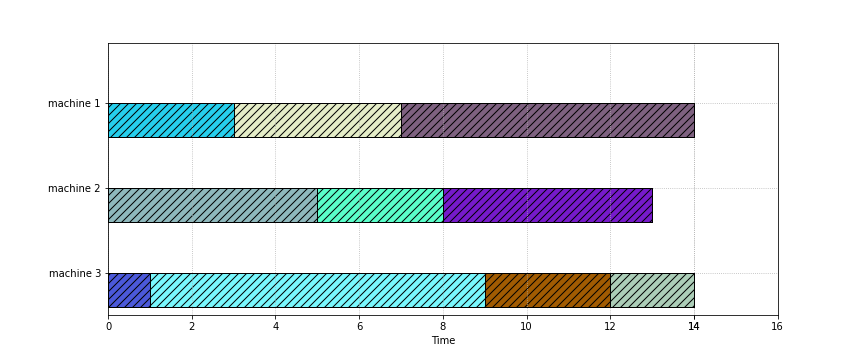
\includegraphics[width=1\textwidth]{PMS}
			\end{figure}
		\end{frame}
		\begin{frame}
			\frametitle{Parallel Machine Scheduling Problem}
			\begin{columns}[c]
				\column{0.4\textwidth}
				- \textbf{Sets and Parameters}
				\begin{itemize}
					\item $M$ Set of identical machines.
					\item $J$ Set of jobs, each has a length of process time.
					\item $p_j, \forall j \in J$ The process time for job $j$.
				\end{itemize}				
				- \textbf{Decision Variables:}
				\begin{itemize}
					\item $x_{ij}, \forall j \in J, i \in M$, Binary, $x_{ij} = 1$ if job $j$ is assigned to machine $m$.
					\item $z$ Time span.
				\end{itemize}

				\column{0.6\textwidth}
				- \textbf{Integer Programming Model}
				\begin{align}
					\min \quad & z \label{pms:obj}\\
					\text{s.t.} \quad & z \ge \sum_{j \in J} p_j x_{ij} \quad \forall i \in M\\
					& \sum_{i \in M} x_{ij} = 1 \quad \forall j \in J\\
					& x_{ij} \in \{0, 1\} \quad \forall j \in J, \forall i \in M\\
					& z \ge 0
				\end{align}

				- \textbf{Constraints}
				Each job can assign to one machine once. All jobs needs to be assigned.
			\end{columns}
		\end{frame}

	\section{Traveling Salesman Problem and Callback}
		\begin{frame}
			\frametitle{Traveling Salesman Problem}
			Given a list of cities and the distances between each pair of cities, what is the shortest possible route that visits each city exactly once and returns to the origin city?
			\begin{figure}[!h]
				\centering
				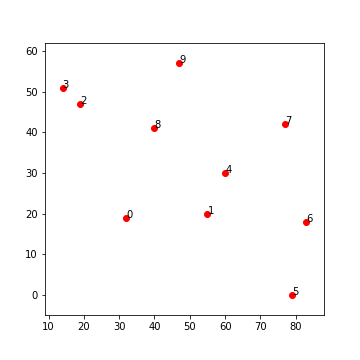
\includegraphics[width=0.5\textwidth]{TSP}
			\end{figure}
		\end{frame}

		\begin{frame}
			\frametitle{Dantzig-Fulkerson-Johnson Formulation}
			let $G = (V, A)$ be a graph where $V$ is a set of $n$ vertices, and $A$ is a set of arcs (or edges). Let $C = c_{ij}$ be a cost (distance) matrix associated with $A$. The TSP consists of determining a minimum cost (distance) Hamiltonian circle (or cycle) that visits each vertex once and only once. If for all $i, j \in V, c_{ij} = c_{ji}$, then the TSP is symmetrical, otherwise is asymmetrical.

			(We use the well-known DFJ formulation)

			- \textbf{Decision variables}
			\begin{equation}
				x_{ij} = \begin{cases}
							1, &\text{if goes from } i \text{ to } j\\ 
							0, & \text{otherwise}
						\end{cases}, \quad (i, j) \in A
			\end{equation}

			- \textbf{Objective function}
				\begin{equation}
					\min \quad \sum_{(i, j)\in A} c_{ij}x_{ij}
				\end{equation}
		\end{frame}

		\begin{frame}
			\frametitle{Dantzig-Fulkerson-Johnson Formulation}
			- \textbf{Constraints}
			\begin{align}
				\sum_{j \in V, (i,j)\in A} x_{ij} & = 1, \quad \forall i \in V \label{TSP:con:degree1}\\
				\sum_{i \in V, (i,j)\in A} x_{ij} & = 1, \quad \forall j \in V \label{TSP:con:degree2}\\
				\sum_{i, j \in S, (i, j) \in A} x_{ij} & \le |S| - 1, \quad \forall S \subset V, 2\le |S| \le n-1\label{TSP:con:DFJSubtour2}
			\end{align}

			If we list all sub-tour constraints in DFJ, there will be $O(2^n)$ constraints and $O(n^2)$ binary variables. The exponential number of constraints makes it impractical to solve directly. Instead, lazy constraints are usually implemented for the sub-tour elimination constraints (\ref{TSP:con:DFJSubtour2})
		\end{frame}

		\begin{frame}
			\frametitle{Subtours}
			In this case, two subtour constraints are identified as 
			\begin{align*}
				x_{14} + x_{49} + x_{97} + x_{76} + x_{65} + x_{51} \le 5\\
				x_{08} + x_{83} + x_{32} + x_{20} \le 3
			\end{align*}

			\begin{figure}[!h]
				\centering
				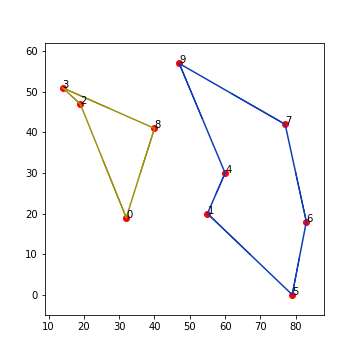
\includegraphics[width=0.5\textwidth]{SubTour}
			\end{figure}
		\end{frame}

		\begin{frame}
			\frametitle{Find subtours}
			\begin{figure}[!h]
				\centering
				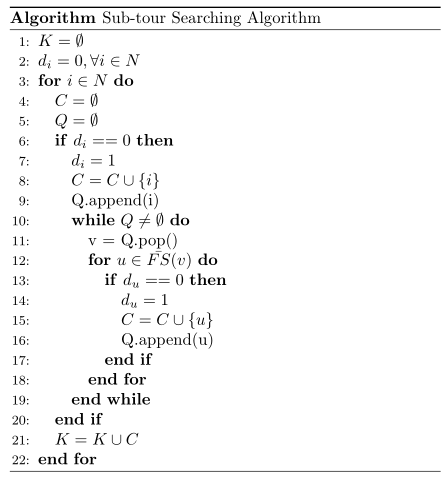
\includegraphics[width=0.6\textwidth]{SubTourAlgo}
			\end{figure}
		\end{frame}

\end{document}